\begin{tikzpicture}
\begin{axis}[height=0.2\textheight,width=0.35\textwidth,style={font=\scriptsize},grid=major,grid style={dotted},align=center,xlabel={Mode},ylabel={Order},title={\ttt{TCL}}, scaled ticks=false, xtick={2,4,6,8,10}, xticklabels={2,4,6,8,10}, ytick={2,4,6,8,10}, yticklabels={2,4,6,8,10}, point meta max=23, point meta min=1, zmin=1, zmax=23, ztick={1,12,23},zticklabels={1,12,23}, zlabel={Gflops/s}, view={-35}{45}, xlabel style={yshift=2mm}, ylabel style={yshift=5mm}, zlabel style={yshift=-1mm,xshift=-4mm}, title style={yshift=-2mm}] % ,
\addplot3[surf] %, colormap = {whiteblack}{color(0cm)=(white);color(0.4cm) = (darkgray)}
coordinates{
(1.000,2.000,22.456) (1.000,3.000,22.094) (1.000,4.000,7.206) (1.000,5.000,7.143) (1.000,6.000,7.285) (1.000,7.000,7.364) (1.000,8.000,7.105) (1.000,9.000,7.222) (1.000,10.000,7.174) 

(2.000,2.000,1.936) (2.000,3.000,1.808) (2.000,4.000,0.727) (2.000,5.000,0.859) (2.000,6.000,1.099) (2.000,7.000,1.588) (2.000,8.000,2.220) (2.000,9.000,2.761) (2.000,10.000,3.681) 

(3.000,2.000,1.920) (3.000,3.000,1.766) (3.000,4.000,0.652) (3.000,5.000,0.755) (3.000,6.000,0.848) (3.000,7.000,1.063) (3.000,8.000,1.485) (3.000,9.000,2.138) (3.000,10.000,2.658) 

(4.000,2.000,1.938) (4.000,3.000,1.745) (4.000,4.000,0.610) (4.000,5.000,0.721) (4.000,6.000,0.783) (4.000,7.000,0.899) (4.000,8.000,1.093) (4.000,9.000,1.501) (4.000,10.000,2.181) 

(6.000,2.000,1.931) (6.000,3.000,1.759) (6.000,4.000,0.613) (6.000,5.000,0.695) (6.000,6.000,0.761) (6.000,7.000,0.867) (6.000,8.000,1.026) (6.000,9.000,1.183) (6.000,10.000,1.628) 

(7.000,2.000,1.913) (7.000,3.000,1.782) (7.000,4.000,0.609) (7.000,5.000,0.701) (7.000,6.000,0.760) (7.000,7.000,0.922) (7.000,8.000,1.072) (7.000,9.000,1.196) (7.000,10.000,1.623) 

(8.000,2.000,1.916) (8.000,3.000,1.758) (8.000,4.000,0.612) (8.000,5.000,0.699) (8.000,6.000,0.765) (8.000,7.000,0.933) (8.000,8.000,1.161) (8.000,9.000,1.270) (8.000,10.000,1.650) 

(9.000,2.000,1.894) (9.000,3.000,1.770) (9.000,4.000,0.608) (9.000,5.000,0.702) (9.000,6.000,0.763) (9.000,7.000,0.922) (9.000,8.000,1.167) (9.000,9.000,1.464) (9.000,10.000,1.687) 

(10.000,2.000,1.915) (10.000,3.000,1.761) (10.000,4.000,0.615) (10.000,5.000,0.705) (10.000,6.000,0.763) (10.000,7.000,0.919) (10.000,8.000,1.149) (10.000,9.000,1.452) (10.000,10.000,2.038) 

};
\end{axis}
\end{tikzpicture}
\begin{comment}
\begin{tikzpicture}
\begin{axis}[height=0.25\textheight,width=0.3\textwidth,style={font=\scriptsize},grid=major,grid style={dotted},align=center,xlabel={Mode},ylabel={Order},title={TCL},scaled ticks=false,zticklabel=\pgfmathprintnumber{\tick},zlabel={Gflops/s},view={-45}{45}, zlabel={Standardfehler [\%]}]
\addplot3[surf]
coordinates{
(1.000,2.000,22.642) (1.000,3.000,15.424) (1.000,4.000,6.600) (1.000,5.000,9.366) (1.000,6.000,6.103) (1.000,7.000,6.326) (1.000,8.000,9.184) (1.000,9.000,6.843) (1.000,10.000,10.211) 

(2.000,2.000,14.252) (2.000,3.000,19.264) (2.000,4.000,37.164) (2.000,5.000,40.227) (2.000,6.000,51.492) (2.000,7.000,47.107) (2.000,8.000,39.097) (2.000,9.000,38.480) (2.000,10.000,33.946) 

(3.000,2.000,13.449) (3.000,3.000,13.211) (3.000,4.000,19.551) (3.000,5.000,33.191) (3.000,6.000,41.243) (3.000,7.000,50.661) (3.000,8.000,50.632) (3.000,9.000,35.379) (3.000,10.000,32.449) 

(4.000,2.000,15.721) (4.000,3.000,15.754) (4.000,4.000,23.373) (4.000,5.000,32.804) (4.000,6.000,35.998) (4.000,7.000,55.167) (4.000,8.000,57.355) (4.000,9.000,56.130) (4.000,10.000,37.866) 

(6.000,2.000,8.194) (6.000,3.000,16.002) (6.000,4.000,22.827) (6.000,5.000,36.494) (6.000,6.000,44.103) (6.000,7.000,54.573) (6.000,8.000,67.934) (6.000,9.000,65.625) (6.000,10.000,62.020) 

(7.000,2.000,10.694) (7.000,3.000,15.072) (7.000,4.000,21.784) (7.000,5.000,37.209) (7.000,6.000,41.483) (7.000,7.000,53.899) (7.000,8.000,64.716) (7.000,9.000,68.793) (7.000,10.000,62.875) 

(8.000,2.000,14.520) (8.000,3.000,16.172) (8.000,4.000,22.225) (8.000,5.000,34.791) (8.000,6.000,42.029) (8.000,7.000,56.385) (8.000,8.000,70.738) (8.000,9.000,73.910) (8.000,10.000,65.133) 

(9.000,2.000,14.687) (9.000,3.000,15.408) (9.000,4.000,22.700) (9.000,5.000,36.494) (9.000,6.000,43.393) (9.000,7.000,54.136) (9.000,8.000,70.710) (9.000,9.000,67.720) (9.000,10.000,63.282) 

(10.000,2.000,14.496) (10.000,3.000,16.808) (10.000,4.000,23.509) (10.000,5.000,36.675) (10.000,6.000,41.853) (10.000,7.000,53.597) (10.000,8.000,66.302) (10.000,9.000,66.482) (10.000,10.000,51.423) 

};
\end{axis}
\end{tikzpicture}
\end{comment}
\hfill
\begin{tikzpicture}
\begin{axis}[height=0.2\textheight,width=0.35\textwidth,style={font=\scriptsize},grid=major,grid style={dotted},align=center,xlabel={Mode},ylabel={Order},title={\ttt{TBLIS}}, scaled ticks=false, xtick={2,4,6,8,10}, xticklabels={2,4,6,8,10}, ytick={2,4,6,8,10}, yticklabels={2,4,6,8,10},  point meta max=11, point meta min=5, zmin=5, zmax=11, ztick={5,8,11},zticklabels={5,8,11}, zlabel={Gflops/s},view={-35}{45}, xlabel style={yshift=2mm}, ylabel style={yshift=5mm}, zlabel style={yshift=-1mm,xshift=-4mm}, title style={yshift=-2mm}]
\addplot3[surf] %, colormap = {whiteblack}{color(0cm)=(white);color(0.4cm) = (darkgray)}
coordinates{
(1.000,2.000,8.056) (1.000,3.000,8.924) (1.000,4.000,9.473) (1.000,5.000,9.750) (1.000,6.000,9.251) (1.000,7.000,9.771) (1.000,8.000,10.006) (1.000,9.000,10.304) (1.000,10.000,9.868) 

(2.000,2.000,6.594) (2.000,3.000,8.123) (2.000,4.000,9.431) (2.000,5.000,9.824) (2.000,6.000,9.122) (2.000,7.000,9.130) (2.000,8.000,9.093) (2.000,9.000,9.135) (2.000,10.000,9.214) 

(3.000,2.000,6.716) (3.000,3.000,5.978) (3.000,4.000,7.856) (3.000,5.000,8.009) (3.000,6.000,7.851) (3.000,7.000,7.794) (3.000,8.000,7.757) (3.000,9.000,7.965) (3.000,10.000,7.945) 

(4.000,2.000,6.619) (4.000,3.000,5.990) (4.000,4.000,7.486) (4.000,5.000,7.580) (4.000,6.000,7.260) (4.000,7.000,7.214) (4.000,8.000,7.220) (4.000,9.000,6.743) (4.000,10.000,7.004) 

(6.000,2.000,6.723) (6.000,3.000,5.868) (6.000,4.000,6.619) (6.000,5.000,6.046) (6.000,6.000,5.970) (6.000,7.000,5.710) (6.000,8.000,5.891) (6.000,9.000,5.823) (6.000,10.000,5.773) 

(7.000,2.000,6.735) (7.000,3.000,5.918) (7.000,4.000,6.923) (7.000,5.000,5.793) (7.000,6.000,6.162) (7.000,7.000,6.069) (7.000,8.000,5.798) (7.000,9.000,5.440) (7.000,10.000,5.408) 

(8.000,2.000,6.712) (8.000,3.000,5.919) (8.000,4.000,6.637) (8.000,5.000,5.662) (8.000,6.000,6.187) (8.000,7.000,5.632) (8.000,8.000,5.838) (8.000,9.000,5.908) (8.000,10.000,5.531) 

(9.000,2.000,6.679) (9.000,3.000,6.169) (9.000,4.000,6.940) (9.000,5.000,5.858) (9.000,6.000,6.013) (9.000,7.000,6.044) (9.000,8.000,5.925) (9.000,9.000,5.838) (9.000,10.000,5.535) 

(10.000,2.000,6.510) (10.000,3.000,5.818) (10.000,4.000,6.465) (10.000,5.000,5.631) (10.000,6.000,5.905) (10.000,7.000,5.480) (10.000,8.000,5.960) (10.000,9.000,5.935) (10.000,10.000,5.795) 


};
\end{axis}
\end{tikzpicture}
\begin{comment}
\begin{tikzpicture}
\begin{axis}[height=0.25\textheight,width=0.3\textwidth,style={font=\scriptsize},grid=major,grid style={dotted},align=center,xlabel={Mode},ylabel={Order},title={TBLIS},scaled ticks=false,zticklabel=\pgfmathprintnumber{\tick},zlabel={Gflops/s},view={-45}{45}, zlabel={Standardfehler [\%]}]
\addplot3[surf]
coordinates{
(1.000,2.000,14.730) (1.000,3.000,8.524) (1.000,4.000,11.426) (1.000,5.000,10.155) (1.000,6.000,6.509) (1.000,7.000,8.492) (1.000,8.000,9.587) (1.000,9.000,10.999) (1.000,10.000,11.072) 

(2.000,2.000,5.945) (2.000,3.000,5.711) (2.000,4.000,6.823) (2.000,5.000,7.575) (2.000,6.000,7.714) (2.000,7.000,8.068) (2.000,8.000,7.474) (2.000,9.000,6.964) (2.000,10.000,7.310) 

(3.000,2.000,5.117) (3.000,3.000,5.224) (3.000,4.000,7.150) (3.000,5.000,6.026) (3.000,6.000,6.899) (3.000,7.000,6.805) (3.000,8.000,7.133) (3.000,9.000,5.931) (3.000,10.000,5.978) 

(4.000,2.000,7.250) (4.000,3.000,5.954) (4.000,4.000,7.465) (4.000,5.000,5.717) (4.000,6.000,3.978) (4.000,7.000,6.547) (4.000,8.000,6.094) (4.000,9.000,13.217) (4.000,10.000,5.921) 

(6.000,2.000,4.515) (6.000,3.000,7.737) (6.000,4.000,6.650) (6.000,5.000,6.805) (6.000,6.000,9.231) (6.000,7.000,13.050) (6.000,8.000,5.949) (6.000,9.000,7.607) (6.000,10.000,9.342) 

(7.000,2.000,3.625) (7.000,3.000,5.911) (7.000,4.000,11.458) (7.000,5.000,12.697) (7.000,6.000,3.434) (7.000,7.000,8.786) (7.000,8.000,6.701) (7.000,9.000,15.042) (7.000,10.000,15.952) 

(8.000,2.000,3.804) (8.000,3.000,2.719) (8.000,4.000,8.299) (8.000,5.000,15.371) (8.000,6.000,2.821) (8.000,7.000,15.637) (8.000,8.000,11.543) (8.000,9.000,6.900) (8.000,10.000,15.249) 

(9.000,2.000,6.272) (9.000,3.000,1.206) (9.000,4.000,5.460) (9.000,5.000,9.223) (9.000,6.000,9.533) (9.000,7.000,4.104) (9.000,8.000,12.228) (9.000,9.000,10.853) (9.000,10.000,16.099) 

(10.000,2.000,9.075) (10.000,3.000,5.961) (10.000,4.000,9.959) (10.000,5.000,15.030) (10.000,6.000,7.924) (10.000,7.000,16.783) (10.000,8.000,10.619) (10.000,9.000,12.958) (10.000,10.000,10.422) 

};
\end{axis}
\end{tikzpicture}
\end{comment}
%\caption{
%\footnotesize Dargestellt sind über die Tensorgröße gemittelten \textbf{Durchsätze in Gflops} der \textbf{Tensor}"=\textbf{Vektor}"=\textbf{Multiplikation}.  Daten sind in \textbf{Floating-Point<Single>} codiert.
%\label{fig:ttv_surf_perf_float}
%}
%\end{figure}
%\clearpage
%\begin{figure}[H]
%\centering
\hfill
\begin{tikzpicture}
\begin{axis}[height=0.2\textheight,width=0.35\textwidth,style={font=\scriptsize},grid=major,grid style={dotted},align=center,xlabel={Mode},ylabel={Order},title={\ttt{EIGEN}}, scaled ticks=false, xtick={2,4,6,8,10}, xticklabels={2,4,6,8,10}, ytick={2,4,6,8,10}, yticklabels={2,4,6,8,10}, point meta max=8, point meta min=2, zmin=2, zmax=8, ztick={2,5,8},zticklabels={2,5,8}, zlabel={Gflops/s},view={-35}{45}, xlabel style={yshift=2mm}, ylabel style={yshift=5mm}, zlabel style={yshift=-1mm,xshift=-4mm}, title style={yshift=-2mm}]
\addplot3[surf] %, colormap = {whiteblack}{color(0cm)=(white);color(0.4cm) = (darkgray)}
coordinates{
%(1.000,2.000,0.614) (1.000,3.000,0.197) (1.000,4.000,0.108) (1.000,5.000,0.086) (1.000,6.000,0.072) (1.000,7.000,0.064) (1.000,8.000,0.056) (1.000,9.000,0.049) (1.000,10.000,0.044) 

(2.000,2.000,7.175) (2.000,3.000,5.427) (2.000,4.000,4.655) (2.000,5.000,4.198) (2.000,6.000,3.577) (2.000,7.000,3.163) (2.000,8.000,2.840) (2.000,9.000,2.556) (2.000,10.000,2.321) 

(3.000,2.000,7.180) (3.000,3.000,6.205) (3.000,4.000,4.718) (3.000,5.000,4.195) (3.000,6.000,3.626) (3.000,7.000,3.193) (3.000,8.000,2.860) (3.000,9.000,2.593) (3.000,10.000,2.328) 

(4.000,2.000,7.204) (4.000,3.000,6.344) (4.000,4.000,5.725) (4.000,5.000,4.136) (4.000,6.000,3.579) (4.000,7.000,3.175) (4.000,8.000,2.827) (4.000,9.000,2.560) (4.000,10.000,2.320) 

(6.000,2.000,7.194) (6.000,3.000,6.332) (6.000,4.000,5.809) (6.000,5.000,3.588) (6.000,6.000,2.866) (6.000,7.000,3.059) (6.000,8.000,2.769) (6.000,9.000,2.533) (6.000,10.000,2.280) 

(7.000,2.000,7.193) (7.000,3.000,6.338) (7.000,4.000,5.711) (7.000,5.000,3.563) (7.000,6.000,2.875) (7.000,7.000,2.311) (7.000,8.000,2.787) (7.000,9.000,2.515) (7.000,10.000,2.280) 

(8.000,2.000,7.216) (8.000,3.000,6.273) (8.000,4.000,5.758) (8.000,5.000,3.539) (8.000,6.000,2.878) (8.000,7.000,2.338) (8.000,8.000,2.016) (8.000,9.000,2.512) (8.000,10.000,2.293) 

(9.000,2.000,7.078) (9.000,3.000,6.337) (9.000,4.000,5.779) (9.000,5.000,3.574) (9.000,6.000,2.886) (9.000,7.000,2.301) (9.000,8.000,2.006) (9.000,9.000,1.735) (9.000,10.000,2.286) 

(10.000,2.000,7.279) (10.000,3.000,6.215) (10.000,4.000,5.712) (10.000,5.000,3.591) (10.000,6.000,2.898) (10.000,7.000,2.313) (10.000,8.000,1.986) (10.000,9.000,1.728) (10.000,10.000,1.593) 

};
\end{axis}
\end{tikzpicture}
\begin{comment}
\begin{tikzpicture}
\begin{axis}[height=0.25\textheight,width=0.3\textwidth,style={font=\scriptsize},grid=major,grid style={dotted},align=center,xlabel={Mode},ylabel={Order},title={EIGEN},scaled ticks=false,zticklabel=\pgfmathprintnumber{\tick},zlabel={Gflops/s},view={-45}{45}, zlabel={Standardfehler [\%]}]
\addplot3[surf]
coordinates{(1.000,2.000,21.045) (1.000,3.000,8.941) (1.000,4.000,7.637) (1.000,5.000,8.191) (1.000,6.000,11.831) (1.000,7.000,10.046) (1.000,8.000,7.536) (1.000,9.000,5.436) (1.000,10.000,2.240) 

(2.000,2.000,1.213) (2.000,3.000,1.924) (2.000,4.000,1.875) (2.000,5.000,0.647) (2.000,6.000,0.626) (2.000,7.000,1.061) (2.000,8.000,1.457) (2.000,9.000,1.710) (2.000,10.000,2.184) 

(3.000,2.000,0.878) (3.000,3.000,0.879) (3.000,4.000,1.410) (3.000,5.000,0.851) (3.000,6.000,1.161) (3.000,7.000,0.767) (3.000,8.000,0.961) (3.000,9.000,1.372) (3.000,10.000,2.241) 

(4.000,2.000,1.929) (4.000,3.000,1.146) (4.000,4.000,1.294) (4.000,5.000,1.482) (4.000,6.000,0.765) (4.000,7.000,0.899) (4.000,8.000,0.972) (4.000,9.000,0.854) (4.000,10.000,1.347) 

(6.000,2.000,1.720) (6.000,3.000,1.466) (6.000,4.000,2.151) (6.000,5.000,1.361) (6.000,6.000,1.122) (6.000,7.000,2.041) (6.000,8.000,1.296) (6.000,9.000,1.556) (6.000,10.000,1.812) 

(7.000,2.000,0.925) (7.000,3.000,0.944) (7.000,4.000,1.543) (7.000,5.000,1.445) (7.000,6.000,0.789) (7.000,7.000,1.095) (7.000,8.000,1.196) (7.000,9.000,1.898) (7.000,10.000,2.490) 

(8.000,2.000,0.896) (8.000,3.000,1.725) (8.000,4.000,1.662) (8.000,5.000,0.850) (8.000,6.000,1.125) (8.000,7.000,0.669) (8.000,8.000,0.951) (8.000,9.000,1.220) (8.000,10.000,2.128) 

(9.000,2.000,1.074) (9.000,3.000,1.326) (9.000,4.000,1.561) (9.000,5.000,0.988) (9.000,6.000,1.093) (9.000,7.000,0.579) (9.000,8.000,1.268) (9.000,9.000,0.749) (9.000,10.000,1.605) 

(10.000,2.000,1.100) (10.000,3.000,1.411) (10.000,4.000,1.012) (10.000,5.000,0.820) (10.000,6.000,0.869) (10.000,7.000,0.777) (10.000,8.000,0.849) (10.000,9.000,0.781) (10.000,10.000,19.561) 

};
\end{axis}
\end{tikzpicture}
\end{comment}
%\caption{
%\footnotesize Dargestellt sind über die Tensorgröße gemittelten \textbf{Durchsätze in Gflops} der \textbf{Tensor}"=\textbf{Vektor}"=\textbf{Multiplikation}.  Daten sind in \textbf{Floating-Point<Single>} codiert.
%\label{fig:ttv_surf_perf_float}
%}
%\end{figure}
